\documentclass{article}
\usepackage[utf8]{inputenc}
\usepackage[a4paper,top=1.5cm,bottom=1.5cm,left=3cm,right=3cm,marginparwidth=1.75cm]{geometry}
\usepackage{natbib}
\usepackage{graphicx}
\usepackage{amsmath, amsthm, amssymb, amsfonts}
\usepackage{titlesec}
\usepackage{makecell}
\usepackage{inconsolata}
\usepackage{tikz}
\usepackage{caption, copyrightbox}
\captionsetup{justification=centering, labelfont=sc, labelsep=endash}
\usepackage{minted}
\usetikzlibrary{automata,positioning}
\usetikzlibrary{arrows}
\usetikzlibrary{shapes}
\definecolor{blue(pigment)}{rgb}{0.2, 0.2, 0.6}
\definecolor{blue(ryb)}{rgb}{0.01, 0.28, 1.0}
\definecolor{brightcerulean}{rgb}{0.11, 0.67, 0.84}
\definecolor{emerald}{rgb}{0.31, 0.78, 0.47}
\tikzset {
        recnode/.style={align=center,inner sep=0pt, rectangle, text width=5cm, draw,thick,minimum width=5cm,minimum height=1cm},
        default/.style={}
}
\makeatletter
\@addtoreset{subsection}{section}
\@addtoreset{subsection}{*section}
\makeatother
\def\thesubsection{\arabic{subsection}}

\let\oldsection\section
\renewcommand{\section}{%
    \setcounter{subsection}{0}%
    \oldsection%
}


\title{Computer Networks - HW1}
\author{Alireza Rostami \\ Student Number: 9832090}
\date{}

\begin{document}
    \maketitle
    
    \section*{Question 1}
    There are seven layers in the OSI model. The layers are shown in the picture below: \\
    \bigskip
    \begin{center}
        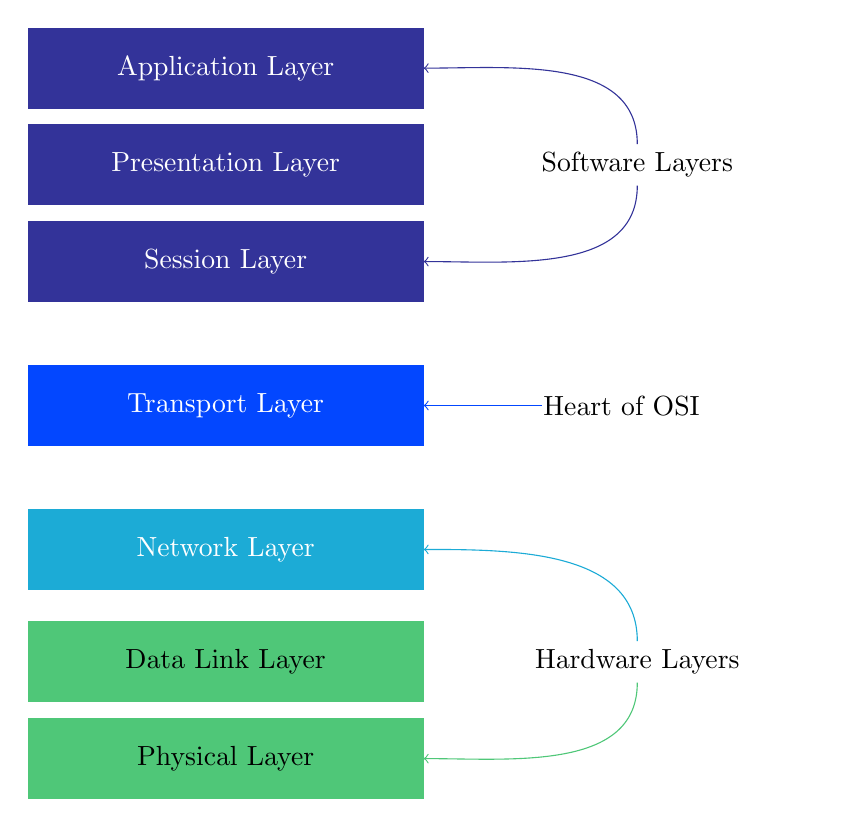
\begin{tikzpicture}[every node/.style=recnode]
            \node[white, draw=blue(pigment), fill=blue(pigment)] (ApplicationLayer) at (0,0) {
                Application Layer
            };
            \node[below=2mm of ApplicationLayer, white, draw=blue(pigment), fill=blue(pigment)] (PresentationLayer) {
                Presentation Layer
            };
            \node[below=2mm of PresentationLayer, white, draw=blue(pigment), fill=blue(pigment)] (SessionLayer) {
                Session Layer
            };
            \node[below=8mm of SessionLayer, white, draw=blue(ryb), fill=blue(ryb)] (TransportLayer) {
                Transport Layer
            };
            \node[below=8mm of TransportLayer, white, draw=brightcerulean, fill=brightcerulean] (NetworkLayer) {
                Network Layer
            };
            \node[below=4mm of NetworkLayer, black, draw=emerald, fill=emerald] (DataLinkLayer) {
                Data Link Layer
            };
            \node[below=2mm of DataLinkLayer, black, draw=emerald, fill=emerald] (PhysicalLayer) {
                Physical Layer
            };
            \node[right=2mm of PresentationLayer, black, draw=white, fill=white, text width=5cm, draw,thick,minimum width=5cm,minimum height=5mm] (SoftwareLayers) {
                Software Layers
            };
            \node[right=15mm of TransportLayer, default, rectangle, draw=white, fill=white, text width=2cm, draw,thick,minimum width=2cm,minimum height=5mm] (Heart) {
                Heart of OSI
            };
            \node[right=2mm of DataLinkLayer, black, draw=white, fill=white, text width=5cm, draw,thick,minimum width=5cm,minimum height=5mm] (HardwareLayers) {
                Hardware Layers
            };
            
            \draw[->] (SoftwareLayers) edge [out=90, in=0, blue(pigment)] (ApplicationLayer);
            \draw[->] (SoftwareLayers) edge [out=-90, in=0,  blue(pigment)] (SessionLayer);
            
            \draw[->] (Heart) edge [out=-180, in=0,  blue(ryb)] (TransportLayer);
            
            \draw[->] (HardwareLayers) edge [out=+90, in=0, brightcerulean] (NetworkLayer);
            \draw[->] (HardwareLayers) edge [out=-90, in=0, emerald] (PhysicalLayer);
        \end{tikzpicture}
    \end{center}
    \subsection{Application Layer}
    At the very top of the OSI Reference Model stack of layers, we find the Application layer which is implemented by the end-user applications. These applications, such as web browsers and email clients, receive by or send over the data, using the network. This layer also serves as a window for the application services to present meaningful data to users.
    
    \subsection{Presentation Layer}
    The presentation layer prepares data for the application layer. It defines how two devices should encode, encrypt, and compress data so it is received correctly on the other end. The presentation layer takes any data transmitted by the application layer and prepares it for transmission over the session layer.
    Examples of its functions:
    \begin{itemize}
        \item \textbf{Translation}: For example, ASCII to EBCDIC.
        \item \textbf{Encryption/Decryption}: Data encryption translates the data into another form or code. The encrypted data is known as the ciphertext and the decrypted data is known as plain text. A key value is used for encrypting as well as decrypting data.
        \item \textbf{Compression}: Reduces the number of bits that need to be transmitted on the network.
    \end{itemize}
    
    \subsection{Session Layer}
    The session layer creates communication channels, called sessions, between devices. It is responsible for opening sessions, ensuring they remain open and functional while data is being transferred, and closing them when communication ends. The session layer can also set checkpoints during a data transfer if the session is interrupted, devices can resume data transfer from the last checkpoint. \\ \\
    The functions of the session layer are:
    \begin{itemize}
        \item \textbf{Session establishment, maintenance, and termination}: The layer allows the two processes to establish, use and terminate a connection.
        \item \textbf{Synchronization}: This layer allows a process to add checkpoints which are considered synchronization points into the data. These synchronization points help to identify the error so that the data is re-synchronized properly, and ends of the messages are not cut prematurely and data loss is avoided.
        \item \textbf{Dialog controller}: The session layer allows two systems to start communication with each other in half-duplex or full-duplex.
    \end{itemize}
    \subsection{Transport Layer}
    The transport layer takes data transferred in the session layer and breaks it into “segments” on the transmitting end. It is responsible for reassembling the segments on the receiving end, turning it back into data that can be used by the session layer. The transport layer carries out flow control, sending data at a rate that matches the connection speed of the receiving device, and error control, checking if data was received incorrectly and if not, requesting it again. \\ \\
    The functionality of the transport layer is:
    \begin{itemize}
        \item \textbf{At sender’s side:} Transport layer receives the formatted data from the upper layers, performs segmentation, and also implements flow \& error control to ensure proper data transmission. It also adds source and destination port numbers in its header and forwards the segmented data to the Network layer. 
        \item \textbf{At receiver’s side:} Transport layer reads the port number from its header and forwards the data which it has received to the respective application. It also performs sequencing and reassembling of the segmented data.
    \end{itemize}
    The functions of the transport layer are:
    \begin{itemize}
        \item \textbf{Segmentation and Reassembly}: This layer accepts the message from the (session) layer, and breaks the message into smaller units. Each of the segments produced has a header associated with it. The transport layer at the destination station reassembles the message.
        \item \textbf{Service Point Addressing}: In order to deliver the message to the correct process, the transport layer header includes a type of address called service point address or port address. Thus by specifying this address, the transport layer makes sure that the message is delivered to the correct process.
    \end{itemize}
    
    \subsection{Network Layer}
    The network layer has two main functions. One is breaking up segments into network packets, and reassembling the packets on the receiving end. The other is routing packets by discovering the best path across a physical network. The network layer uses network addresses (typically Internet Protocol addresses) to route packets to a destination node.
    The functions of the network layer are:
    \begin{itemize}
        \item \textbf{Routing}: The network layer protocols determine which route is suitable from source to destination. This function of the network layer is known as routing.
        \item \textbf{Logical Addressing}: In order to identify each device on internetwork uniquely, the network layer defines an addressing scheme. The sender \& receiver’s IP addresses are placed in the header by the network layer. Such an address distinguishes each device uniquely and universally.
    \end{itemize}

    \subsection{Data Link Layer}
    The data link layer establishes and terminates a connection between two physically-connected nodes on a network. It breaks up packets into frames and sends them from source to destination. This layer is composed of two parts—Logical Link Control (LLC), which identifies network protocols, performs error checking and synchronizes frames, and Media Access Control (MAC) which uses MAC addresses to connect devices and define permissions to transmit and receive data.
    The functions of the data link layer are:
    \begin{itemize}
        \item \textbf{Framing}: Framing is a function of the data link layer. It provides a way for a sender to transmit a set of bits that are meaningful to the receiver. This can be accomplished by attaching special bit patterns to the beginning and end of the frame.
        \item \textbf{Physical addressing}: After creating frames, the Data link layer adds physical addresses (MAC address) of the sender and/or receiver in the header of each frame.
        \item \textbf{Error control}: Data link layer provides the mechanism of error control in which it detects and retransmits damaged or lost frames.
        \item \textbf{Flow control}: The data rate must be constant on both sides else the data may get corrupted thus, flow control coordinates the amount of data that can be sent before receiving acknowledgement.
        \item \textbf{Access control}: When a single communication channel is shared by multiple devices, the MAC sub-layer of the data link layer helps to determine which device has control over the channel at a given time.
    \end{itemize}

    \subsection{Physical Layer}
    The lowest layer of the OSI reference model is the physical layer. The physical layer is responsible for the physical cable or wireless connection between network nodes. It defines the connector, the electrical cable or wireless technology connecting the devices, and is responsible for transmission of the raw data, which is simply a series of 0s and 1s, while taking care of bit rate control.
    The functions of the data link layer are:
    \begin{itemize}
        \item \textbf{Bit synchronization}: The physical layer provides the synchronization of the bits by providing a clock. This clock controls both sender and receiver thus providing synchronization at bit level.
        \item \textbf{Bit rate control}: The Physical layer also defines the transmission rate i.e. the number of bits sent per second.
        \item \textbf{Physical topologies}: Physical layer specifies the way in which the different, devices/nodes are arranged in a network i.e. bus, star, or mesh topology.
        \item \textbf{Transmission mode}: Physical layer also defines the way in which the data flows between the two connected devices. The various transmission modes possible are simplex, half-duplex and full-duplex.
    \end{itemize}
     ~\\ Answer was retrieved from
    \begin{itemize}
        \item \textsl{GeeksforGeeks. (2022c, June 15). Layers of OSI Model. \\ https://www.geeksforgeeks.org/layers-of-osi-model}
        \item \textsl{What is OSI Model $|$ 7 Layers Explained. (2020, June 10). Learning Center. \\ https://www.imperva.com/learn/application-security/osi-model/}
    \end{itemize}
    and expanded upon.
    \pagebreak
    \section*{Question 2}
    \subsection{Transmission delay} The time taken to transmit a packet from the host to the transmission medium is called transmission delay. For example, if bandwidth is 1 bps (every second 1 bit can be transmitted onto the transmission medium) and the data size is 20 bits then 20 seconds would be required. 
    For the general formula, suppose $ B $ bps is the bandwidth and $L$ bit is the size of the data. Therefore, transmission delay is:
    \begin{equation}
        T_t = \frac{L}{B}
    \end{equation}
    ~\\This delay depends upon the following factors:
    \begin{itemize}
        \item If there are multiple active sessions, the delay will become significant.
        \item Increasing bandwidth decreases transmission delay.
        \item MAC protocol largely influences the delay if the link is shared among multiple devices.
        \item Sending and receiving a packet involves a context switch in the operating system, which takes a finite time.
    \end{itemize}
    
    \subsection{Propagation delay}
    After the packet is transmitted to the transmission medium, it has to go through the medium to reach the destination. Hence the time taken by the last bit of the packet to reach the destination is called propagation delay. 
    The factors affecting propagation delay are:
    \begin{itemize}
        \item \textbf{Distance}: It takes more time to reach the destination if the distance of the medium is longer. 
        \item \textbf{Velocity}: If the velocity(speed) of the signal is higher, the packet will be received faster.
    \end{itemize}
    Let $D$ be the distance and $V$ be the speed of the signal. The formula for propagation delay is:
    \begin{equation}
        T_p = \frac{D}{V} 
    \end{equation}
    
    \subsection{Queueing delay}
    After the packet is received by the destination, it will not be processed by the destination immediately. It has to wait in a queue in something called a buffer. So the amount of time it waits in queue before being processed is called queueing delay. \\
    In general, we are not able to calculate queueing delay because there is not a general formula for that. 
    ~\\This delay depends upon the following factors:
    \begin{itemize}
        \item If the size of the queue is large, the queuing delay will be huge. If the queue is empty there will be less or no delay.
        \item If more packets are arriving in a short or no time interval, queuing delay will be large.
        \item The less the number of servers/links, the greater is the queuing delay.
    \end{itemize}
    
    \subsection{Processing delay}
    Now the packet will be taken for the processing which is called processing delay.

    Time is taken to process the data packet by the processor that is the time required by intermediate routers to decide where to forward the packet, update TTL, perform header checksum calculations.
    
     It also does not have any general formula since it depends upon the speed of the processor.
     
     In conclusion, the total delay is the sum of all delays.
     Therefore:
     \begin{equation}
         T_{total} = T_t + T_p + T_q + T_{pro} \approx T_t + T_p.
     \end{equation}

    \section*{Question 3}
    Two ISPs at the same level of the hierarchy often peer with each other to send and receive traffic directly and avoid paying to the intermediate ISP provider. If two ISP's do not peer with each other, then they need an intermediate ISP provider to send traffic to each other.
    
    ~\\IXP can earn money by charging each ISP that connects to it. The IXP charges each ISP based on the amount of traffic sent to or received from the IXP.

    \section*{Question 5}
    Traceroute is a network diagnostic tool used to track in real-time the pathway taken by a packet on an IP network from source to destination, reporting the IP addresses of all the routers it pinged in between. Traceroute also records the time taken for each hop the packet makes during its route to the destination.
    It can be easily used. For example, in Windows, you may type:
    \texttt{tracert <Name of the website>}.
    
    \section*{Question 6}
    IP spoofing is the creation of Internet Protocol (IP) packets which have a modified source address in order to either hide the identity of the sender, to impersonate another computer system, or both. It is a technique often used by bad actors to invoke DDoS attacks against a target device or the surrounding infrastructure.\\
    
    \begin{figure}[!h]
        \centering
        \copyrightbox[b]{\includegraphics[scale=0.23]{images/ip-spoofing.png}}{How IP spoofing works \\Courtesy of Cloudflare}
    \end{figure}
    
    \pagebreak
    \section*{Question 7}
    Hexagonal cells means each cell has six neighbors.
    \begin{center}
        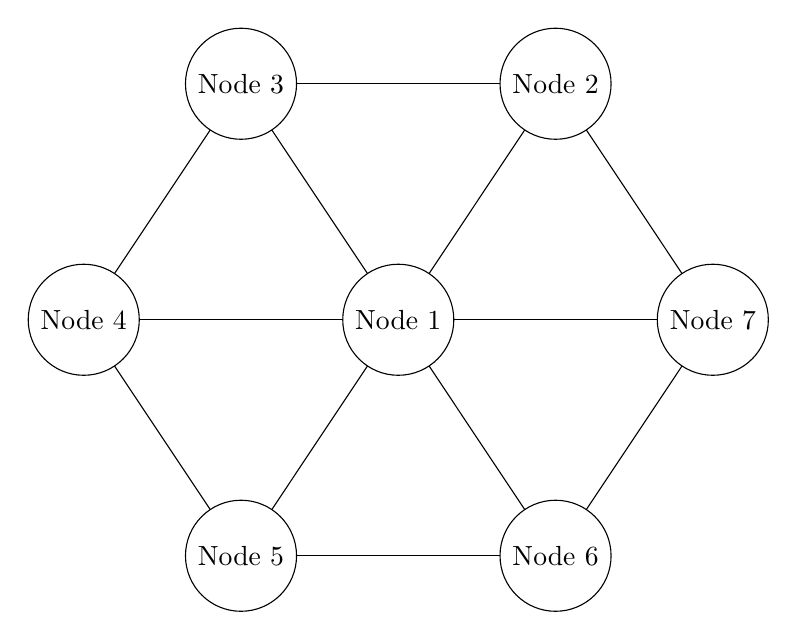
\begin{tikzpicture}
            \begin{scope}[%
                every node/.style={anchor=west,
                circle,
                draw,
                radius = 5cm,
                outer sep=0,
            },
            transform shape]
    \node (A) {Node 1};
    \node (B)[above right = 20mm and 10mm of A] {Node 2};
    \node (C)[above left = 20mm and 10mm of A] {Node 3};
    \node (D)[below right = 20mm and 10mm of B]{Node 7};
    \node (E)[below left = 20mm and 10mm of C] {Node 4};
    \node (F)[below right = 20mm and 10mm of A]  {Node 6};
    \node (G)[below left = 20mm and 10mm of A] {Node 5};
    
    \draw[-] (A) edge (B);
    \draw[-] (A) edge (C);
    \draw[-] (C) edge (B);
    \draw[-] (C) edge (E);
    \draw[-] (E) edge (G);
    \draw[-] (G) edge (F);
    \draw[-] (D) edge (F);
    \draw[-] (D) edge (B);
    \draw[-] (D) edge (A);
    \draw[-] (F) edge (A);
    \draw[-] (E) edge (A);
    \draw[-] (A) edge (G);

            
  \end{scope}
\end{tikzpicture}

    \end{center}

    If the central cell uses frequency  $ A $, its six neighbors can use $ B $, $C$, $B$, $C$, $B$, and $C$ respectively. Think of this as a graph-coloring problem. This graph can be colored with 3 colors. In other words, only 3 unique cells are needed. Consequently, each cell would have $ \frac{840}{3}= 280$.

    
    \section*{Question 8}
    If the algorithm is changed for the operations at layer $ k $, the services at $k+1$ will change since the services will be operated after the layer. For the services at $k-1$, they will not be affected since they are prior to the algorithms.
    
    \section*{Question 9}
    The delay of the circuit-switched network is $ s + k \cdot d + \frac{x}{b}$. The delay of the packet-switched network is $T_{total} = T_{Transmition} + T_{Propagation} + T_{Queueing} + T_{Processing}$ for entire message, plus delay incurred in re-transmitting the last bit (k-1) times: $ k \cdot d + \frac{x}{b} + (k-
1) \cdot \frac{p}{b}$ where we assume for simplicity that x is divisible by p.
Therefore, the circuit-switched network has a lower delay if $s < (k-1)\cdot \frac{p}{b}$.
Informally, the call setup delay must be less than the transmission delays
stemming from repeated forwarding in the store-and-forward operations. Notice that it does not depend on x, since all intermediate routers can forward packets in
parallel.

\section*{Question 10}
At time $t_0$ the sending host begins to transmit. At time $t_1 = \frac{L}{R_1}$ the sending host completes transmission and the entire packet is received at the router (no propagation delay). Because the router has the entire packet at time $t_1$ it can begin to transmit the packet to the receiving host at time $t_1$. At time $t_2 = t_1 + \frac{L}{R_2}$ the router completes transmission and the entire packet is received at the receiving host (again, no propagation delay). Thus, the end-to-end delay is $\frac{L}{R_1} + \frac{L}{R_2}$.

\section*{Question 11}
Each telephone makes $ 0.6 $ calls per hour at $ 5 $ minutes each. Therefore, a telephone occupies a circuit for $ 3 $ minutes per hour. $ 20 $ telephones can share a circuit, although having the load be close to $100\%$ ($\rho = 1$ in queuing terms) implies very long wait times. Since $20\%$ of the calls are long-distance, it takes $400$ telephones to occupy a long-distance circuit full time. The interoffice trunk has $\frac{1,000,000}{4000} = 250$ circuits multiplexed onto it. With $400$ telephones per circuit, an end office can support $400 \times 250 = 100,000$ telephones.


\end{document}
